\documentclass{article}

% if you need to pass options to natbib, use, e.g.:
% \PassOptionsToPackage{numbers, compress}{natbib}
% before loading nips_2016
%
% to avoid loading the natbib package, add option nonatbib:
% \usepackage[nonatbib]{nips_2016}

% \usepackage{nips_2016}

% to compile a camera-ready version, add the [final] option, e.g.:
%\usepackage[final]{nips_2016}

\usepackage[utf8]{inputenc} % allow utf-8 input
\usepackage[T1]{fontenc}    % use 8-bit T1 fonts
\usepackage{hyperref}       % hyperlinks
\usepackage{url}            % simple URL typesetting
\usepackage{booktabs}       % professional-quality tables
\usepackage{amsfonts}       % blackboard math symbols
\usepackage{nicefrac}       % compact symbols for 1/2, etc.
\usepackage{microtype}      % microtypography
\usepackage{graphicx}	% graphics
\usepackage{hyperref}	% biblio?

\title{Solving the Heat Equation with Neural Networks}

% The \author macro works with any number of authors. There are two
% commands used to separate the names and addresses of multiple
% authors: \And and \AND.
%
% Using \And between authors leaves it to LaTeX to determine where to
% break the lines. Using \AND forces a line break at that point. So,
% if LaTeX puts 3 of 4 authors names on the first line, and the last
% on the second line, try using \AND instead of \And before the third
% author name.

\author{
  Alexander Havrilla \& Alden Pritchard\\
  Carnegie Mellon University\\
  Pittsburgh, PA 15213 \\
  \texttt{alumhavr@andrew.cmu.edu; atpritch@andrew.cmu.edu} \\
  %% examples of more authors
  %% \And
  %% Coauthor \\
  %% Affiliation \\
  %% Address \\
  %% \texttt{email} \\
  %% \AND
  %% Coauthor \\
  %% Affiliation \\
  %% Address \\
  %% \texttt{email} \\
  %% \And
  %% Coauthor \\
  %% Affiliation \\
  %% Address \\
  %% \texttt{email} \\
  %% \And
  %% Coauthor \\
  %% Affiliation \\
  %% Address \\
  %% \texttt{email} \\
}

\begin{document}
% \nipsfinalcopy is no longer used

\maketitle

\section{Introduction}
The Deep Galerkin Method was first proposed in 2018 by Justin Sirignano and Konstantinos Spiliopoulos, who used the method to numerically solve the Black-Scholes partial differential equation (PDE) for options pricing. This main advantage of the DGM is that it is mesh-free, and as a result does not suffer from the curse of dimensionality, allowing us to compute values in feasible time for higher-dimensional setups. Sirignano and Spiliopoulos proved rigorously that using a deep neural network, as the number of layers goes to infinity, the network approximation converges point wise to the true solution. This is done by choosing a loss function which consists of distance from some initial condition, distance from some boundary condition, and distance from the size of the differential operator applied to the function. By minimizing the sum of these three terms, the method aims to generate a function which closely approximates the initial condition, boundary condition, and a solution on the interior of the domain, thereby giving a numerical solution to the PDE.

\section{Background}

General commentary

2, 3, 7, 4

\subsection{PDEs and Heat Equation}

Partial differential equations, or PDEs, define a subset of differential equations where derivatives with respect to different variables exist in the same equation. PDE's are commonly found in nature as they can describe many different kinds of diffusion processes. For example, the heat equation describes the diffusion of heat in a specified number of dimensions. In the one-dimensional case, there does exist a closed-form analytical solution to the heat equation. However, in the 2-D and more general multivariate case, no analytical solution is known to exist. As a result, if we wish to know how heat will diffuse in a given area under some specified initial conditions, then we need to find an approximation to the heat equation.

\subsection{Traditional Approximation Methods}

Traditional PDE approximation methods involve creating a mesh over the domain of the problem. In the 1-D case, this amounts to breaking the domain interval into some set of $n$ evenly-spaced points. At each point the PDE is approximated as an ODE with initial conditions satisfying the original PDE and then solved numerically at each point in time. When each of these discrete solutions is taken as a whole, we get an approximate solution to the PDE. \\ \\
This process of meshing the domain from a continuous problem into a discrete set of problems and solving the individual ODEs requires a significant amount of both work and approximations, both of which contribute to making solving PDEs very numerically challenging. Since the number of mesh points increases exponentially in the dimension of the problem, it is necessary to use either a smaller domain or a larger distance between mesh points if we want to solve the PDE in a reasonable amount of time. However, as the distance between mesh points increases, the stability of the approximation breaks down. Likewise, restricting the size of the domain yields less information about PDE than we may want. This trade-off demonstrates the difficulty in numerically solving PDEs, as we are forced to choose between runtime and accuracy.\\ \\
Some common methods for discretizing PDEs include Galerkin Methods, Finite Difference Methods, Finite Volume Methods, and Gradient Discretization Methods, among others. Galerkin Methods seek to approximate the PDE using a linear combination of basis functions. In this paper we use Finite Difference Methods for the 1-D case and Finite Volume Methods for the 2-D case in our approximations.\\

\section{Related Work}

Solving PDEs using the DGM architecture was originally proposed by Sirignano and Spiliopoulos in 2018. The authors realized that neural networks were similar in concept to Galerkin Methods through the use of linear combinations of basis functions to approximate some function. Whereas the Galerkin method uses a single linear combination of basis functions to approximate the PDE solution, the DGM uses multiple layers of basis functions. The weights for these functions are determined by training the neural network via xstochastic gradient descent with backpropogation, adam optimizer, and momentum. For the loss function, the authors propose using the sum of distances from the boundary, initial, and differential conditions to approximate the error in the solution.
The authors also showed that as the network depth goes to infinity, the neural network approximation converges point-wise to the PDE solution.\\ \\

Black Scholes Paper and Toronto Review(These both come from University of Toronto)

\subsection{ DGM Architecture }
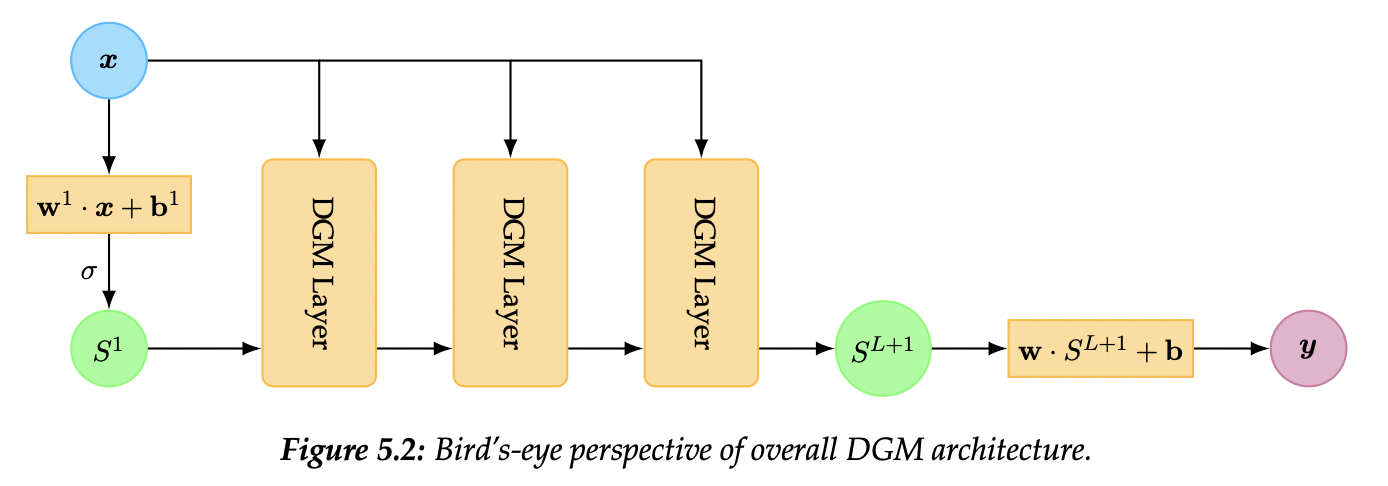
\includegraphics[scale=0.32]{Architecture.png}\\
The overall DGM network architecture consists of a fully connected layer, followed by some number of stacked DGM layers that take as input the original input $x$ and the output of the previous DGM layer, with another fully connected layer at the end. We experimented with different depth networks in anticipation of a trade-off between training time and network accuracy as implied by the results from Sirignano and Spiliopoulos.

\subsection{ Individual DGM layer }
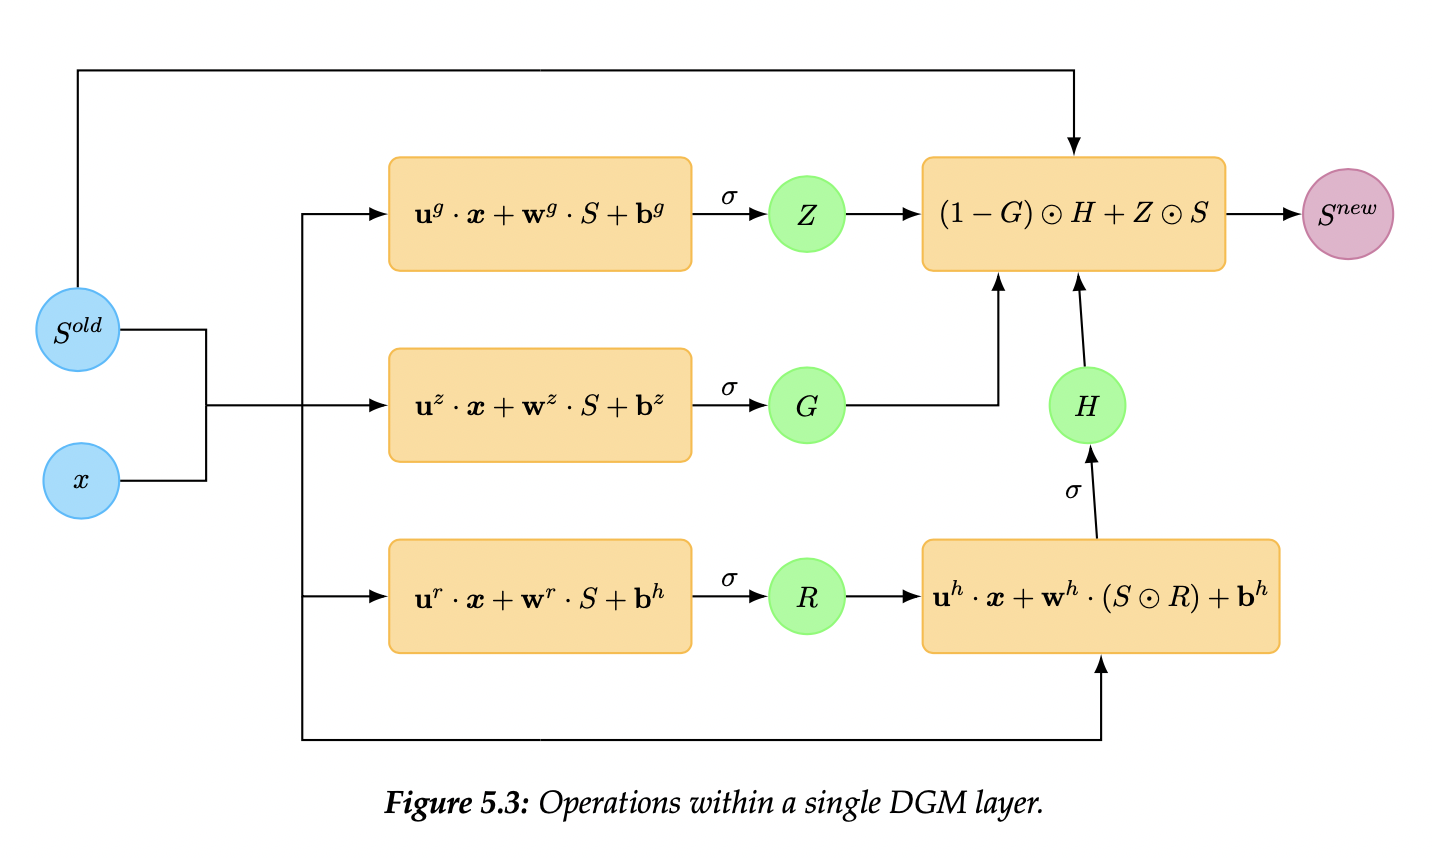
\includegraphics[scale=0.32]{DGM_Layer.png}\\
Each individual DGM layer consists of four sums of linear maps and an output function. In total, each layer contains eight weight matrices, four bias vectors, and four activation functions, which are eventually combined in the layer's output function.

\section{Methods}

General Commentary

\subsection{Architecture}

\subsection{Sampling Methodology}

\subsection{Initial/Boundary Conditions}

\section{Results}

General Commentary

\subsection{Depth of Network}

\subsection{Number of Samples}

\subsection{Dependence on Dimension}

\subsection{Dependence on Initial/Boundary Conditions}


\section{Analysis}

\subsection{Depth of Network}

\subsection{Training Time}

\subsection{Number of Samples}

\subsection{Dependence on Dimension}

\subsection{Dependence on Initial Conditions}

How these things affect time and accuracy?

\section{Future Work}

General Commentary

\subsection{Different Architectures}

\subsection{Dealing Higher Dimensions}

\subsection{Other PDEs}

\section*{References}

References follow the acknowledgments. Use unnumbered first-level
heading for the references. Any choice of citation style is acceptable
as long as you are consistent. It is permissible to reduce the font
size to \verb+small+ (9 point) when listing the references. {\bf
  Remember that you can use a ninth page as long as it contains
  \emph{only} cited references.}
\medskip

\small

[1] Al-Aradi A. Correia A. Naiff D. Jardim G. Solving Nonlinear High-Dimensional Partial Differential Equations via Deep Learning.

[2] Han. J. Solving High-dimensional PDEs Using Deep Learning. https://www.pnas.org/content/pnas/115/34/8505.full.pdf

[3] Penko V. https://github.com/vitkarpenko/FEM-with-backward-Euler-for-the-heat-equation

[4] Sirignano. J, spiliopoulos K. DGM: A deep learning algorithm for solving partial differential equations. https://arxiv.org/abs/1708.07469




\end{document}
